\section{Introducción a LabMan}

Es este apartado se realiza una breve introducción a \acrfull{labman}, el \acrshort{dms} usado por grupos de investigación como MORElab, Mobility y TransLaw, así como de las tecnologías que lo conforman. Este contexto facilitará la comprensión de los próximos capítulos, además de describir los fundamentos clave para el desarrollo de este proyecto.

\begin{figure}[!htp]
	\centering
	\includegraphics[scale=0.15]{fig/MORElab-logo}
	\caption{Logotipo de MORElab}
\end{figure}

Gestionar la información no siempre es una tarea trivial y más aún cuando hay que tratar con los datos que componen varias entidades como pueden ser, dentro del ámbito de la investigación, los proyectos, investigadores, publicaciones, eventos, etc. La mayoría de los grupos de investigación utilizan sistemas de gestión de contenido tales como Joomla!\cite{joomla}, WordPress\cite{wordpress} o Drupal\cite{drupal} para exponer sus datos. Sin embargo, para extraer la información de estos \acrfullpl{cms} se requieren herramientas externas para llevar a cabo técnicas de análisis de datos. 

Para hacer uso de estas herramientas normalmente hace falta generar documentos adicionales, tales como ficheros \acrfull{csv}, hojas de cálculo, ficheros de texto, generando información redundante, que provoca dificultades a la hora de actualizar los datos y la calidad de los mismos. Esta situación empeora cuando además se disponen de distintas fuentes para la obtención de información, como pueden ser las paginas web personales de los investigadores, en las que se muestran sus logros a lo largo de su carrera, la información financiera gestionada por su propio departamento, etc.

Si es verdad que existen extensiones para que los \acrshort{cms} puedan publicar los datos almacenados en estos sistemas como ficheros \acrfull{rdf}, sin embargo estos no permiten acceder a la información mediante el protocolo \acrshort{sparql}, por lo que no se pueden realizar consultas complejas a entidades externas ni aprovechar las ventajas que se producen por publicarlos siguiendo las prácticas de \acrfull{ld}\cite{ld_benefits}.

\begin{figure}[!htp]
	\centering
	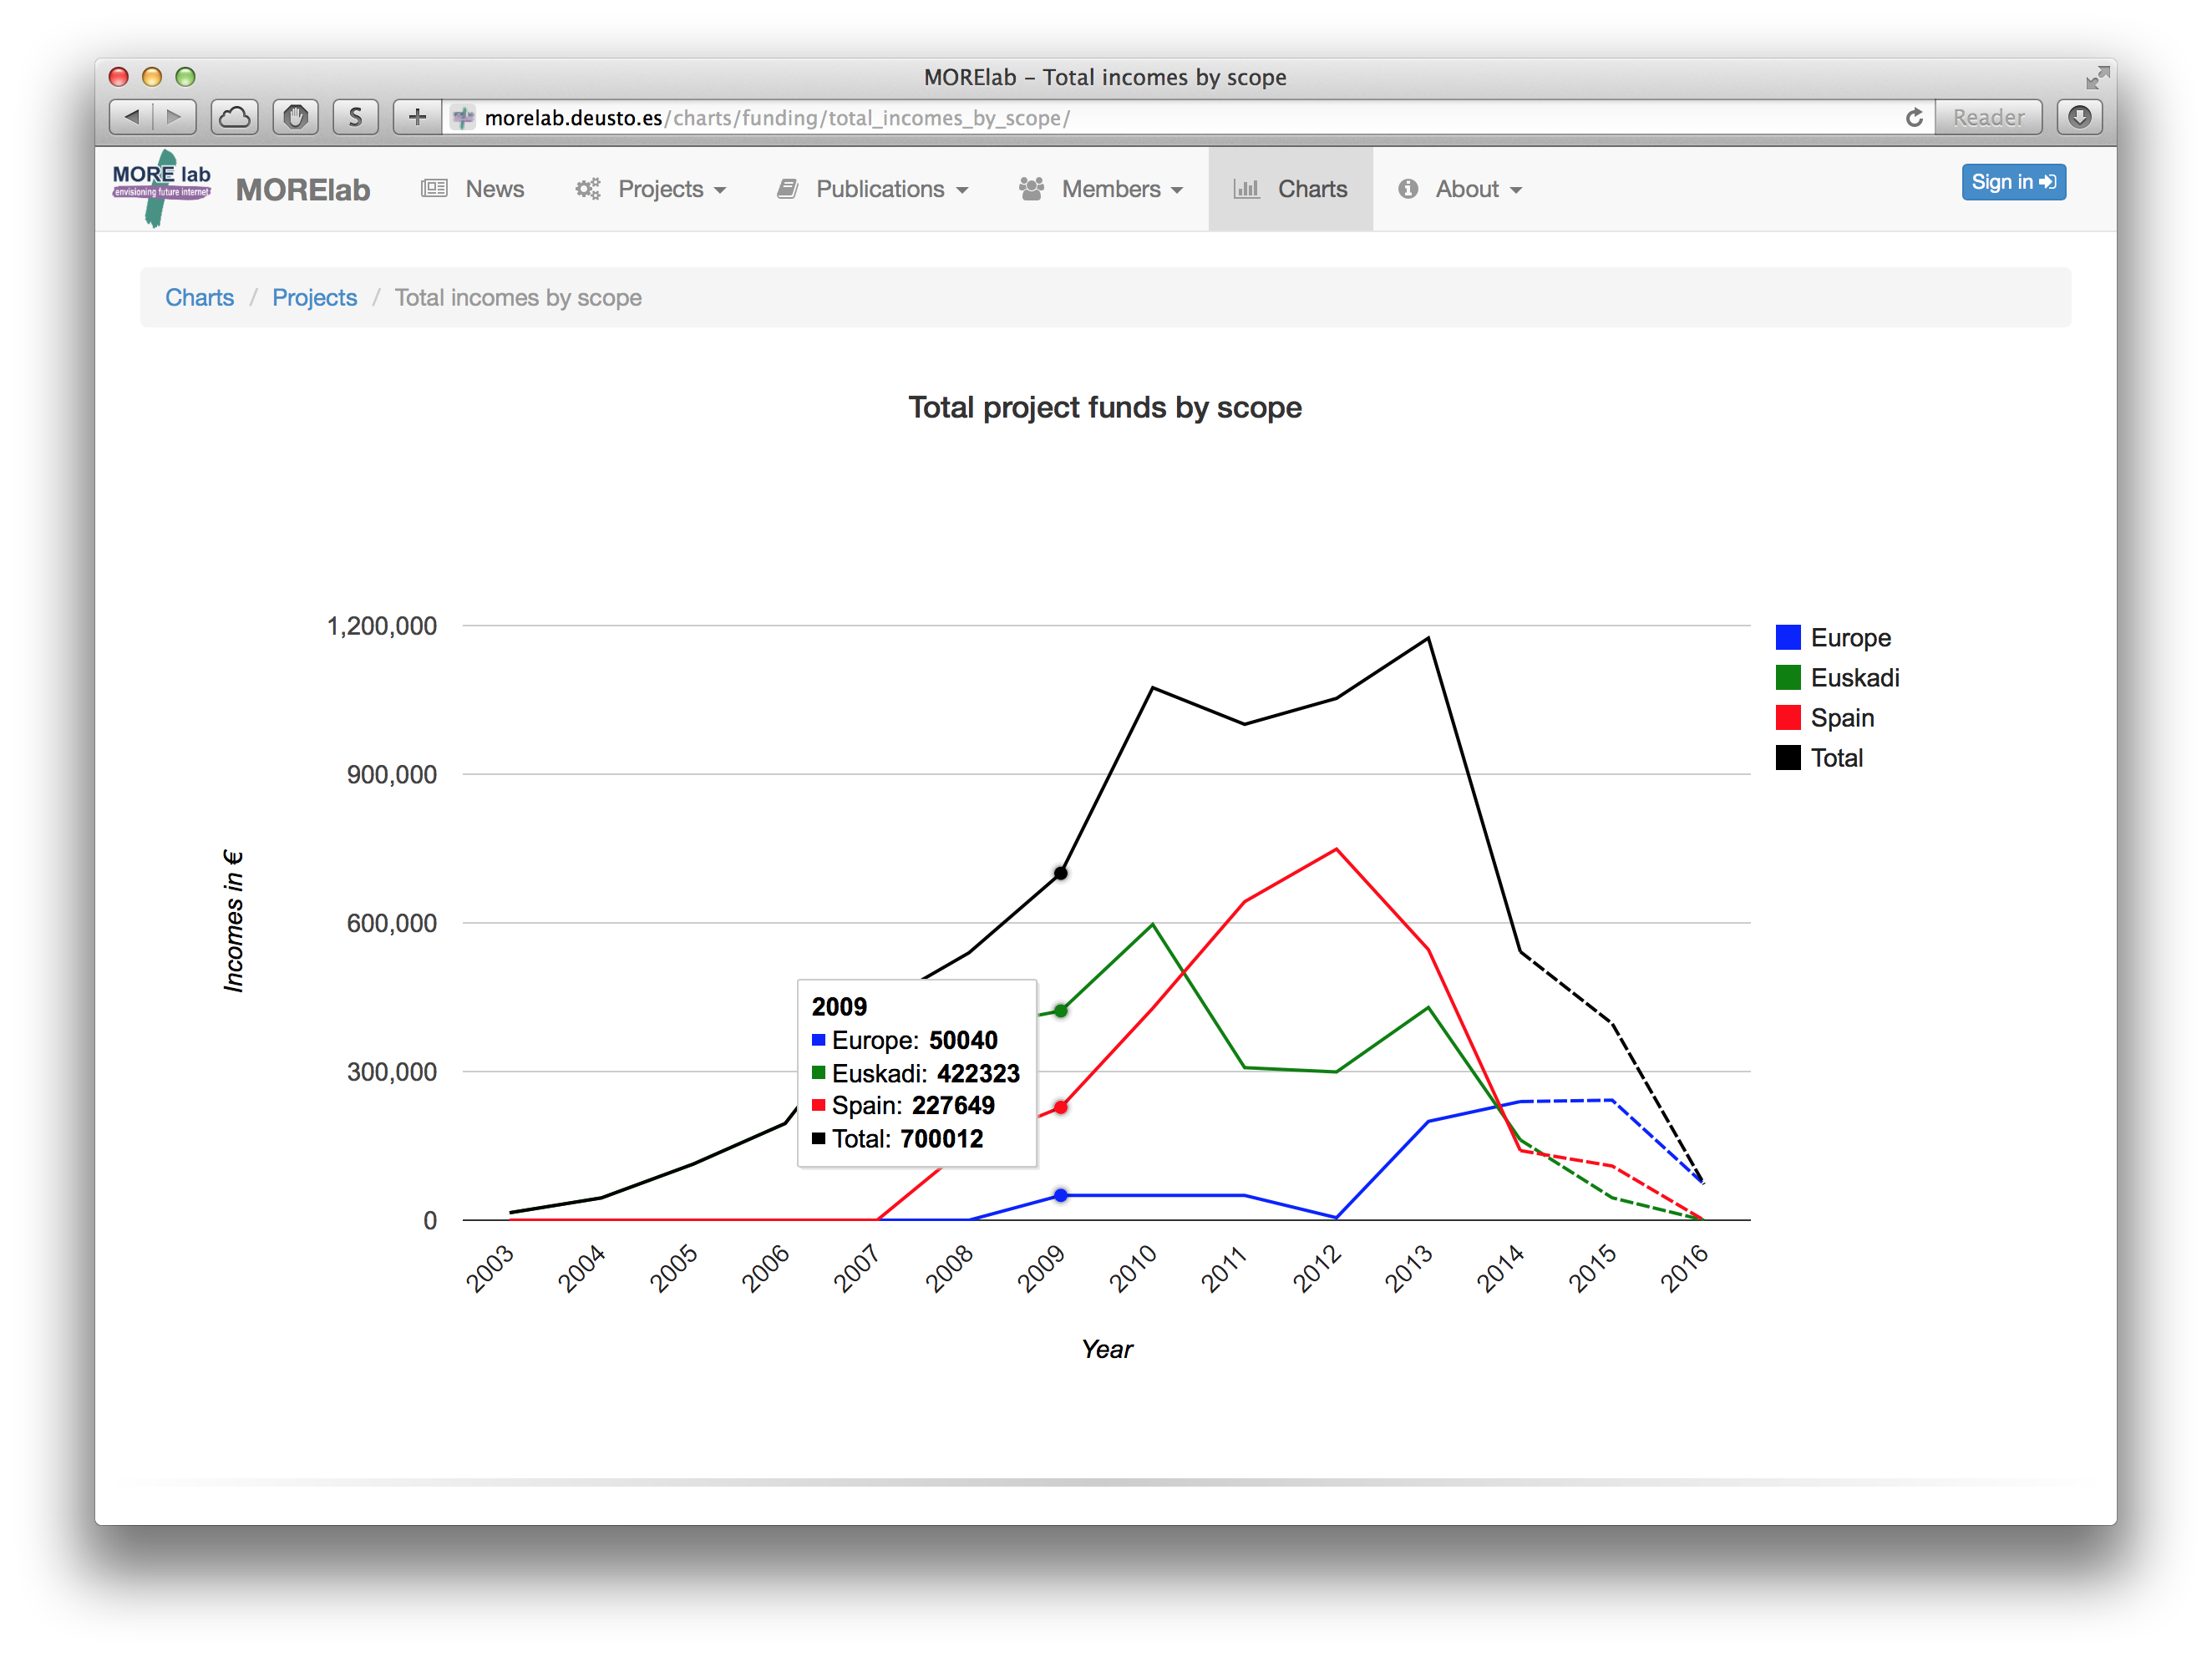
\includegraphics[scale=0.21]{fig/labman-chart}
	\caption{\acrshort{labman}: Gráfico generado por tripletas \acrshort{rdf}}\label{fig:labmanchart}
\end{figure}

Del esfuerzo para gestionar la información del grupo de investigación de MORElab nace \acrshort{labman}, una aplicación desarrollada en Python\cite{Python} por medio del \textit{framework} para desarrollo web Django\cite{Django} que sustituye a la antigua solución Joomla! para la publicación de los datos sobre las publicaciones en \acrfull{rdf}\cite{RDF}. Su principal objetivo es gestionar no solo la información relacionada con las publicaciones, sino que va más allá, publicando la información relacionada a los proyectos del equipo, sus financiaciones e integrantes de proyecto, de una forma gráfica e intuitiva tal y como se puede ver en la figura \ref{fig:labmanchart}, diferenciadose de otros \acrshortpl{cms} por apostar por la exposición de los datos como \acrlong{lod}\cite{linkeddata}, haciendola disponible a todo el mundo sin restricción de derechos de \textit{copyrights} o patentes.\cite{pena_visual_2014}